\documentclass{beamer}[10pt, usepdftitle=false, handout]

\beamertemplatenavigationsymbolsempty

\usepackage[T1]{fontenc}
\usepackage[]{algorithm2e}
\usepackage{multimedia}
\usepackage{gensymb}
\usepackage{textcomp}
\usepackage{color}
%\usepackage{background}
%\backgroundsetup{
%    placement=center,
%    scale=1,
%    contents={The author of this course is PAUL BLONDEL},
%    opacity=0.7
%}
%\setbeamertemplate{background}{\BgMaterial}
%\usepackage[font=small,labelfont=bf]{caption} 
%\usepackage[font=small,labelfont=bf]{caption} 

\usetheme{Boadilla}

\title{Data Structure 4}
\author[]{Paul Blondel}
\institute[]{CNAM}
\date[]{September 1st, 2018}

\usepackage[style=british]{csquotes}


\def\signed #1{{\leavevmode\unskip\nobreak\hfil\penalty50\hskip1em
  \hbox{}\nobreak\hfill #1%
  \parfillskip=0pt \finalhyphendemerits=0 \endgraf}}

\newsavebox\mybox
\newenvironment{aquote}[1]
  {\savebox\mybox{#1}\begin{quote}\openautoquote\hspace*{-.7ex}}
  {\unskip\closeautoquote\vspace*{1mm}\signed{\usebox\mybox}\end{quote}}


%\setbeamertemplate{headline}
%{
%  \leavevmode%
%  \hbox{%
%  \begin{beamercolorbox}[wd=1.0\paperwidth,ht=2.25ex,dp=1ex,center]{author in head/foot}%
%   \textcolor{green}{- This course has been made by Paul Blondel -} \usebeamerfont{author in head/foot}\insertsubsection
%  \end{beamercolorbox}}%
%  \vskip0pt%
%}


\setbeamertemplate{footline}
{
  \leavevmode%
  \hbox{%
  \begin{beamercolorbox}[wd=.5\paperwidth,ht=2.25ex,dp=1ex,center]{author in head/foot}%
    \usebeamerfont{author in head/foot}\insertsection
  \end{beamercolorbox}%
  \begin{beamercolorbox}[wd=.5\paperwidth,ht=2.25ex,dp=1ex,center]{title in head/foot}%
    \usebeamerfont{title in head/foot} \inserttitle \hspace*{2em}  \insertframenumber{} / \inserttotalframenumber\hspace*{2ex} 
  \end{beamercolorbox}}%
  \vskip0pt%
}

\AtBeginSection[]
{
   \begin{frame}
    \tableofcontents[ 
    currentsection] 
   \end{frame}
}
\SetKw{KwBy}{by}

\begin{document}
	{
	\setbeamertemplate{footline}{
  	\leavevmode%
  	\hbox{%
  	\begin{beamercolorbox}[wd=.5\paperwidth,ht=2.25ex,dp=1ex,center]{author in head/foot}%
  	\end{beamercolorbox}%
  	\begin{beamercolorbox}[wd=.5\paperwidth,ht=2.25ex,dp=1ex,center]{title in head/foot}%
  	\end{beamercolorbox}}%
  	\vskip0pt%	
	} 
	\begin{frame}
	\titlepage
	\end{frame}

	\begin{frame}
	
	\begin{aquote}{Linus Torvalds}
	I will, in fact, claim that the difference between a bad programmer and a good one is whether he 
	considers his code or his data structures more important. Bad programmers worry about the code. Good programmers worry about data structures and their relationships.	
	\end{aquote}	
	
	\end{frame}


	\begin{frame}
		\tableofcontents
	\end{frame}
	}

	\addtocounter{framenumber}{-3}

	\section{Trees}	
	\subsection{Definition}

	\begin{frame}[label=(first)]
	
	\begin{block}{What are trees?}
	A tree is a data structure...
	\begin{itemize}
		\item {...with a root element (\textbf{root node})}
		\item {...followed by other elements (or \textbf{nodes}):
			\begin{itemize}
				\item {organized in a \textbf{family of subsets}}
				\item {family subsets organized in \textbf{a tree structure}}
			\end{itemize}
		
		
		}
	\end{itemize}		
	
	\end{block}	
	
	\vspace*{-1em}	
	
	\begin{columns}[c]
	\column{.5\textwidth}
	\begin{center}	
	Example of tree:	
	
	\begin{figure}
		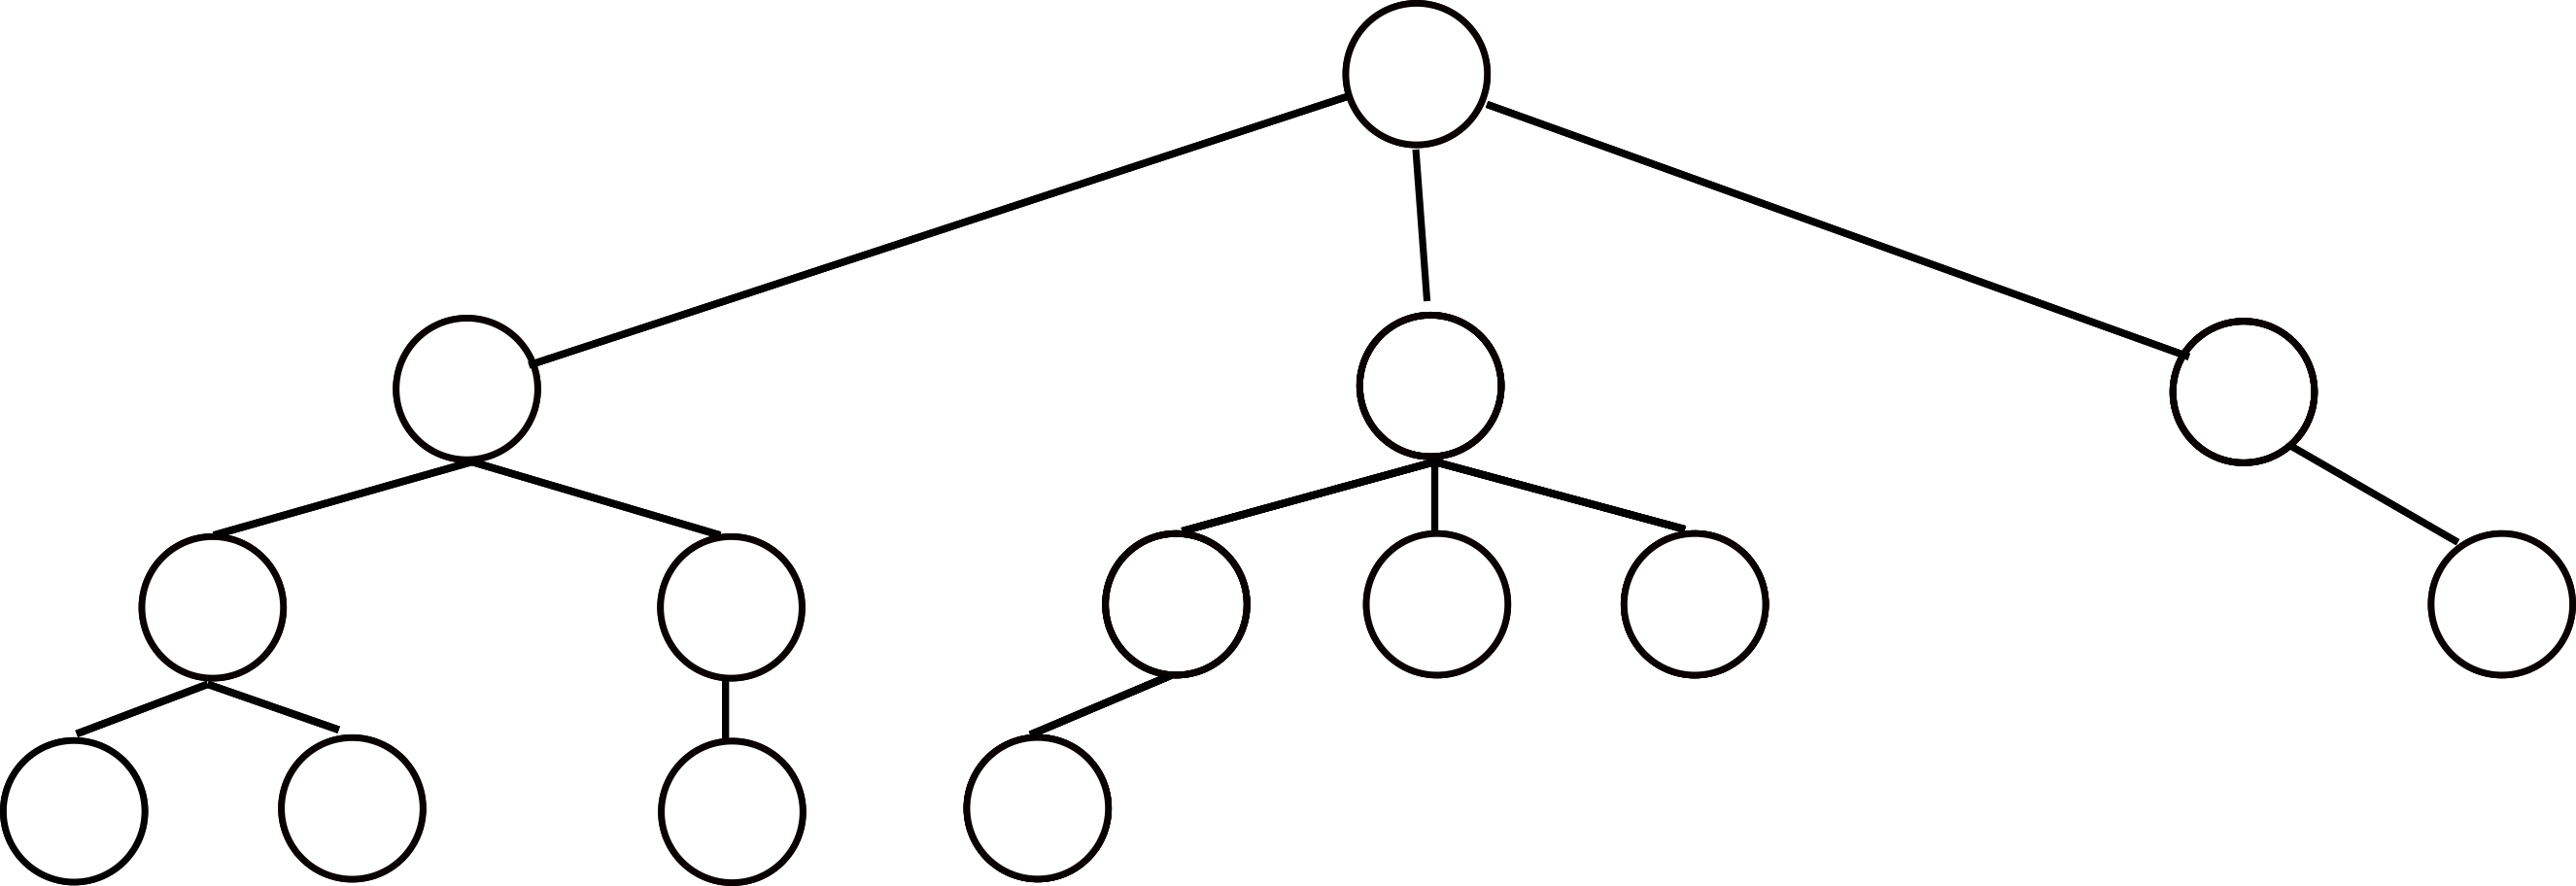
\includegraphics[scale=0.1]{images/trees.png} 
     	%\vspace*{-0.5em}
		%\caption{Floating gate transistor cell}
	\end{figure}		
	\end{center}	
	\column{.5\textwidth}
	\begin{center}
	
	Not all nodes have the same name...	
	\begin{figure}
		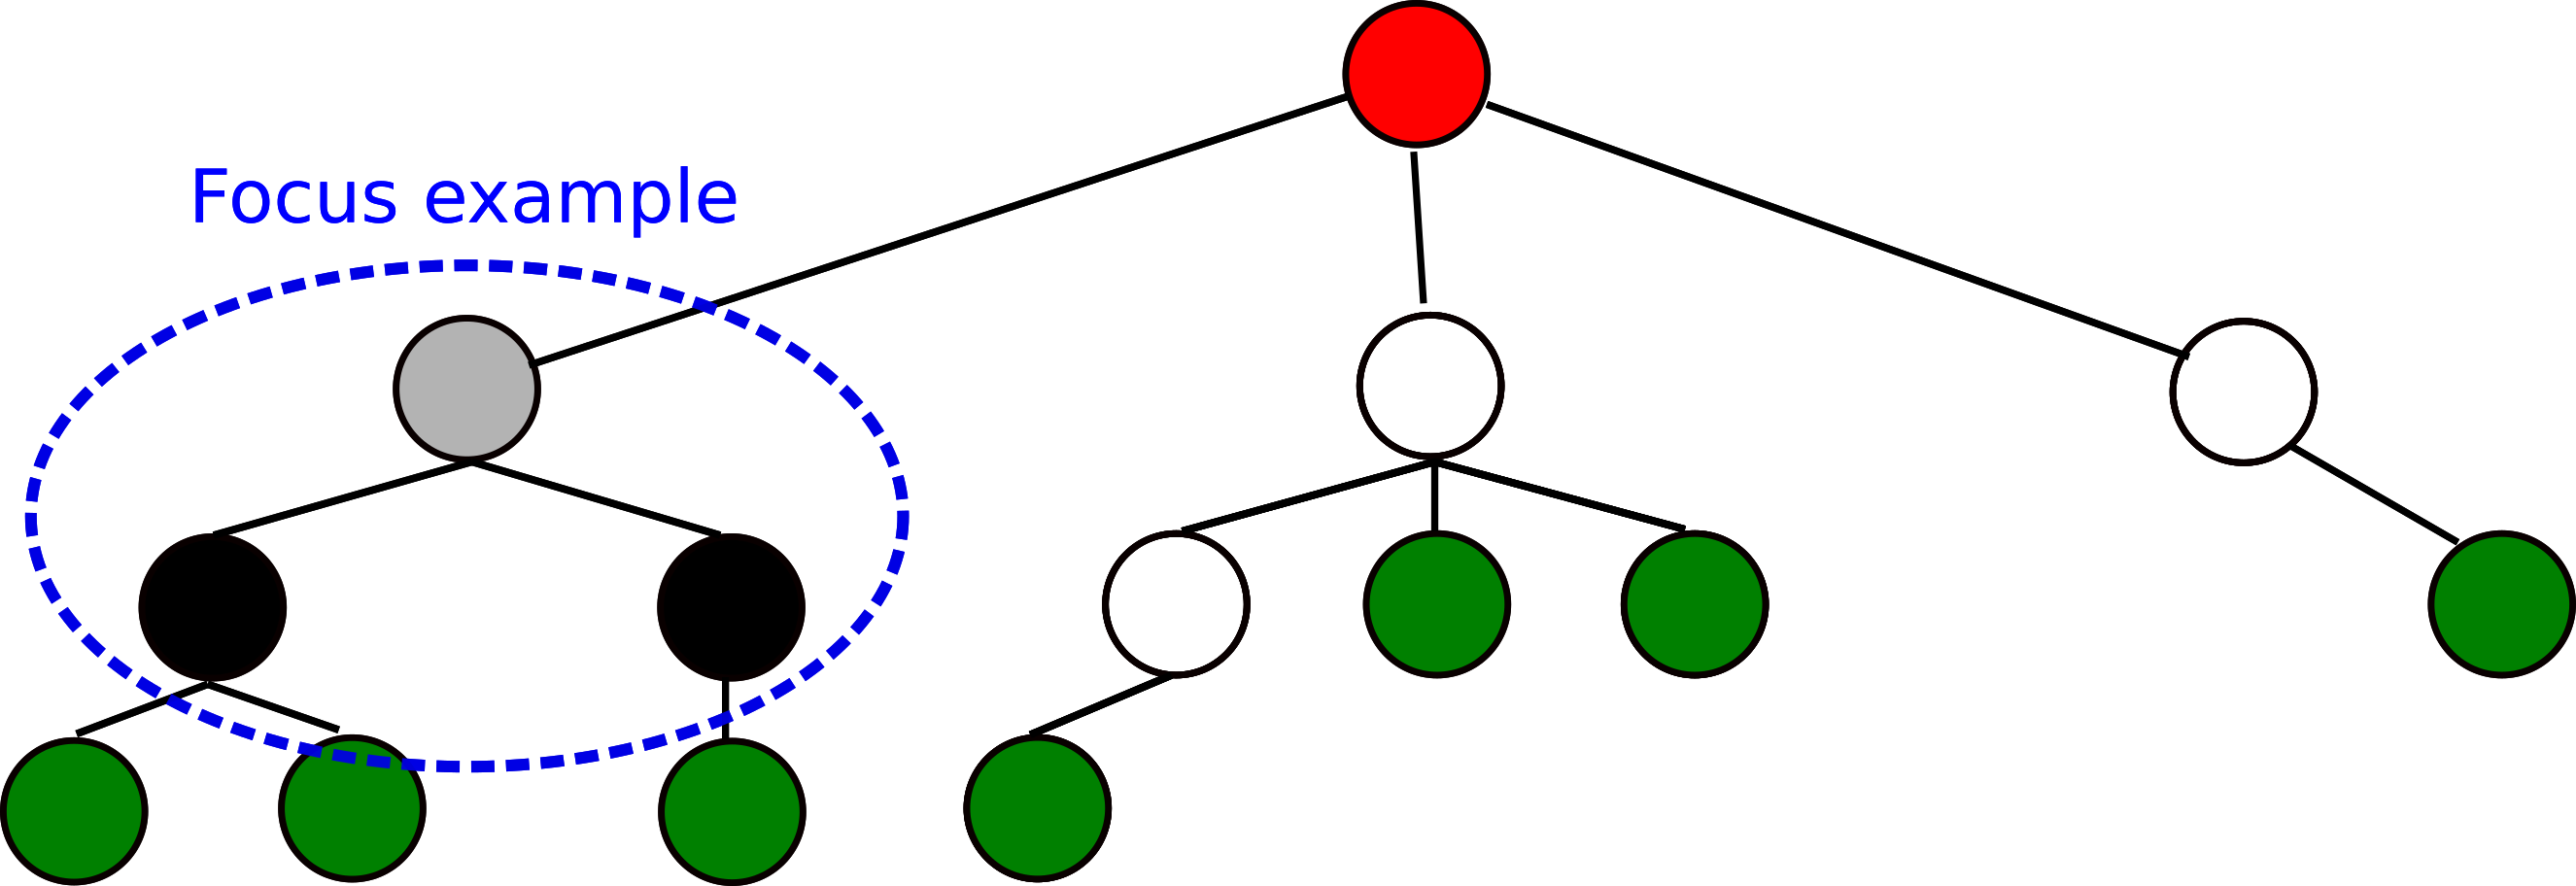
\includegraphics[scale=0.1]{images/trees_vocab.png} 
     	%\vspace*{-0.5em}
		%\caption{Floating gate transistor cell}
	\end{figure}		
	\end{center}	
	\end{columns}
	
	\vspace*{1em}
	
	\begin{itemize}
	\item {In \textit{red}: the \textbf{root node} (\textit{super parent})}
	\item {In \textit{green}: the \textbf{node leaves} (like a leaf of a tree...)}
	\item {Focus example: a parent node (\textit{grey}) with two children nodes (\textit{black})} 	
	\end{itemize}		
	
	\end{frame}

	
	
	\subsection{Traversing and reading a tree}
	
	\begin{frame}
		
	Trees can be traversed in \textbf{\textit{depth-first} or \textit{breadth-first}}\footnotemark[3] order:
	
	\vspace*{1em}
	\begin{itemize}
	\item {\textit{depth-first order}: \textbf{traverse to deepest levels} before other children}
	\item {\textit{breadth-first order}: all nodes are traversed \textbf{level after level}}
	\end{itemize}
	
	\vspace*{1em}
	\textit{Depth-first} traversal (left side) and \textit{breadth-first} traversal (right side):	
	
	\vspace*{1em}
	\begin{figure}
		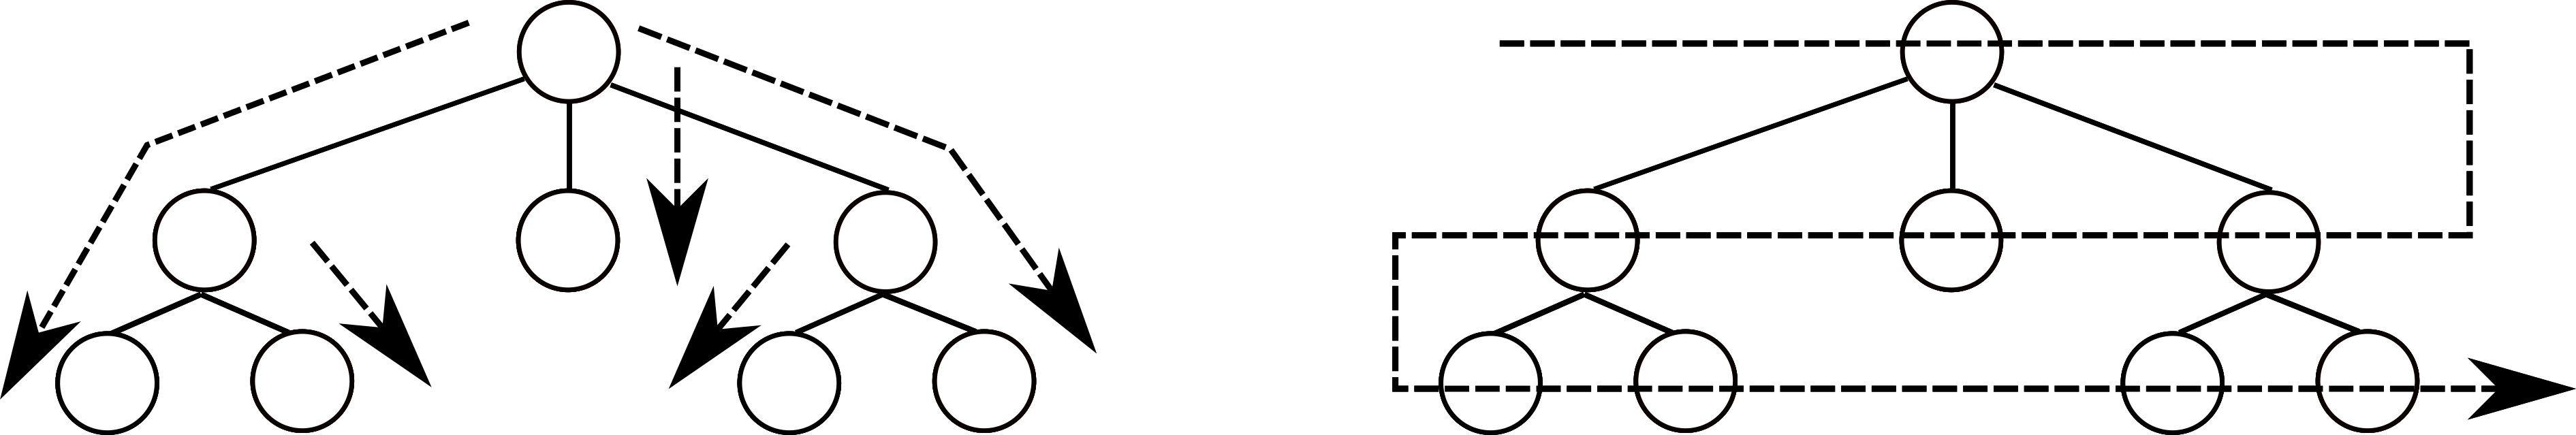
\includegraphics[scale=0.18]{images/trees_traversal.png} 
     	%\vspace*{-0.5em}
		%\caption{Floating gate transistor cell}
	\end{figure}	
		
	\footnotetext[3]{We won't talk much about \textit{breadth-first} order traversal, as it is less used.}	
	
	\end{frame}	
	
	\begin{frame}
	
	Three ways of \textit{reading node contents} with \textit{depth-first} traversal\footnotemark[3]:
	
	\vspace*{1em}
	\begin{itemize}
	\item {\textit{Pre-order}: directly read the \textbf{visited node content}

	
	
	
	}
	\item {\textit{In-order}: traverse \textbf{left subtree and read visited node content}}
	\item {\textit{Post-order}: traverse \textbf{all subtrees and read visited node content}}	
	\end{itemize}
	
	Examples:
	
	\begin{figure}
		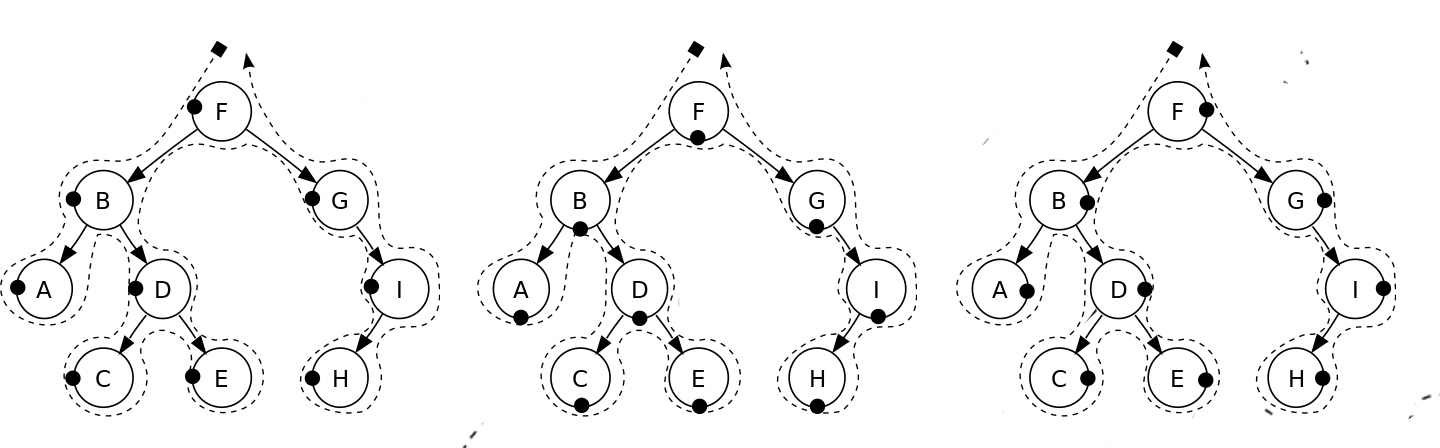
\includegraphics[scale=0.22]{images/traversal_order.png} 
     	%\vspace*{-0.5em}
		%\caption{Floating gate transistor cell}
	\end{figure}	
	
	\pause	
	
	\vspace*{-1em}	
	
	\begin{itemize}
	\item {Left: F, B, A, D, C, E, G, I, H (pre-order)}
	\item {Center: A, B, C, D, E, F, G, H, I (in-order)}
	\item {Right: A, C, E, D, B, H, I, G, F (post-order)}
	\end{itemize}
		
	\footnotetext[3]{By default, node contents are read in \textit{pre-order} mode}
		
	\end{frame}
	
	\section{Binary trees}
	
	\subsection{Properties}
		
	\begin{frame}

	\begin{block}{Binary?}
	\begin{itemize}
	\item {Binary trees are trees with \textbf{\textit{at most} two children} per node}\footnotemark[2]
	\item {A binary tree is a \textbf{special case} of trees}\footnotemark[2]
	\end{itemize}	
	\end{block}
	
	Example of a binary tree (right side: implementation representation):
	\begin{figure}
		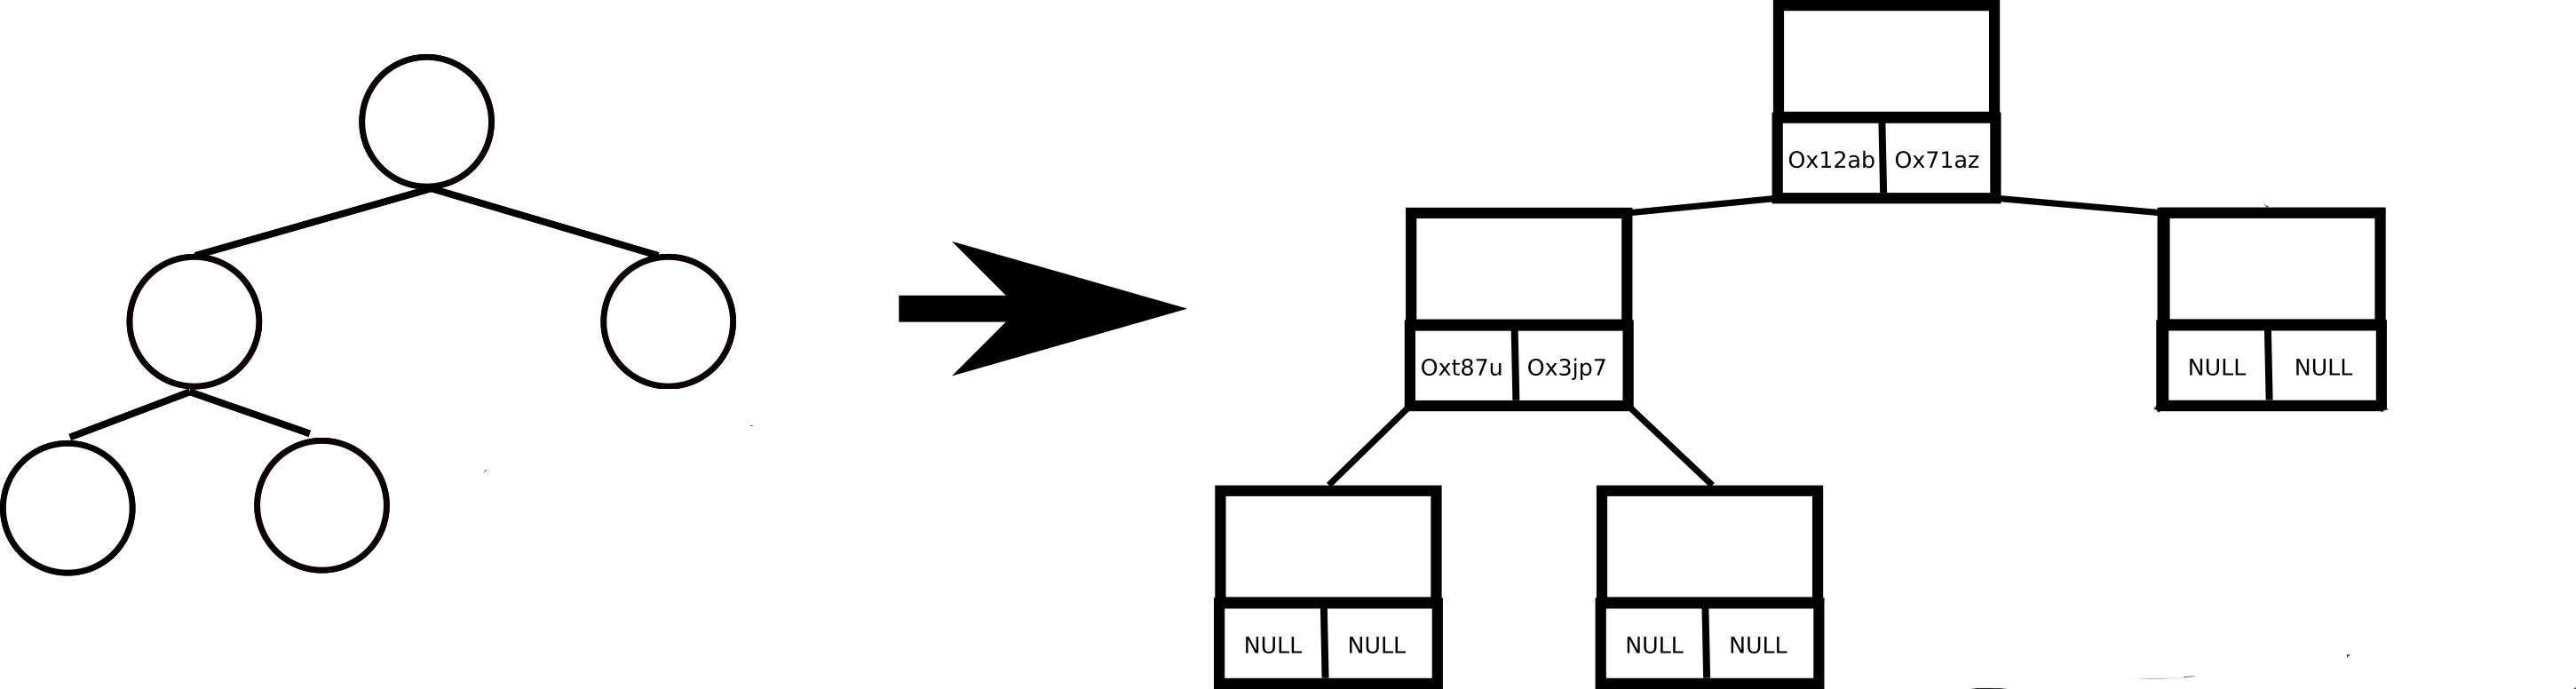
\includegraphics[scale=0.2]{images/binary_trees.png} 
     	%\vspace*{-0.5em}
		%\caption{Floating gate transistor cell}
	\end{figure}	
	
	
	\footnotetext[2]{In Data Structure 3, we briefly talked about binary trees for heap sort}
			
	\end{frame}	
	
	
	\subsection{Complete and almost complete binary trees}	
		
	\begin{frame}
		
	A \textit{binary tree} is said \textit{complete} if...
	
	\begin{itemize}
		\item {... it is a \textbf{binary tree} (of course)}
		\item {... it has \textbf{\textit{$2^k -1$} nodes} ($k$ being the \textit{binary tree high})}				
	\end{itemize}
		
	\vspace*{1em}		
		
	Example:
	
	\begin{figure}
		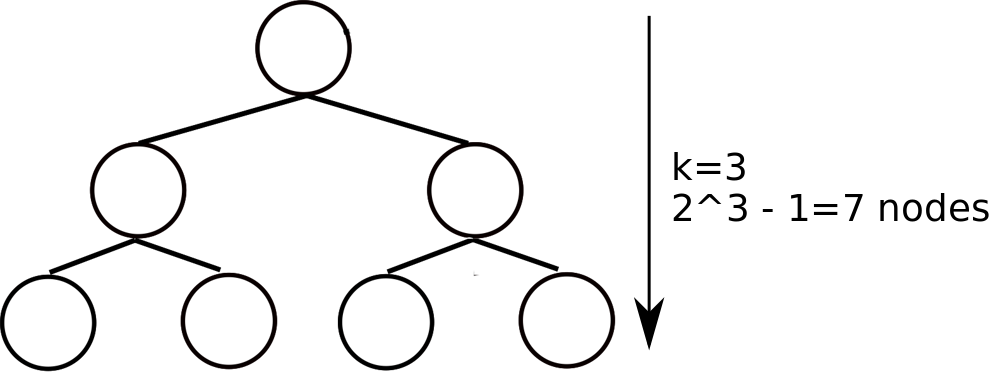
\includegraphics[scale=0.2]{images/binary_tree.png} 
     	%\vspace*{-0.5em}
		%\caption{Floating gate transistor cell}
	\end{figure}	
			

		
	\end{frame}			
	
	\begin{frame}
	
	A binary tree is said \textit{almost complete} if...
	\begin{itemize}
	\item {... it is a \textbf{binary tree}}
	\item {... all levels are complete \textbf{except the last}}
	\item {... the last level being \textbf{partially complete on the \textit{left}}}	
	\end{itemize}		
	
	\vspace*{1em}	
	
	Example:
	\begin{figure}
		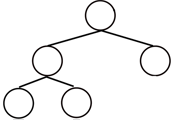
\includegraphics[scale=0.6]{images/binary_tree_p.png} 
     	%\vspace*{-0.5em}
		%\caption{Floating gate transistor cell}
	\end{figure}
		
	
	\end{frame}
	
	\begin{frame}
	
	\begin{block}{Why this data structure is interesting?}
	\textit{Complete} and \textit{almost complete} trees \textbf{can be represented as arrays}:
	\begin{itemize}
	\item {\textit{left child node value} of node $k$ located at \textit{index $2\times k$} in array}
	\item {\textit{right child node value} of node $k$ located at \textit{index $2\times k + 1$} in the array}
	\end{itemize}		
	\end{block}			
		
	\vspace*{1em}		
		
	Example with a \textit{complete tree}:
	\begin{center}
	\begin{figure}
		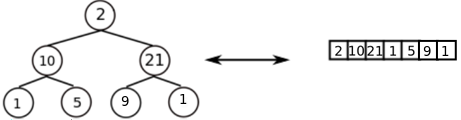
\includegraphics[scale=1.3]{images/binary_tree_array.png} 
     	%\vspace*{-0.5em}
		%\caption{Floating gate transistor cell}
	\end{figure}
	\end{center}	
	
	Example with an \textit{almost complete tree}:
	\begin{center}
	\begin{figure}
		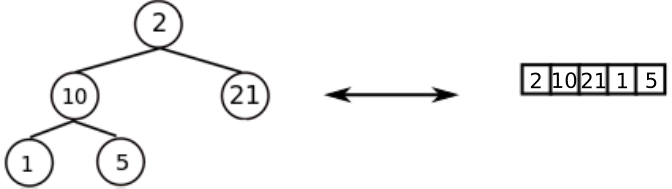
\includegraphics[scale=0.5]{images/binary_tree_p_array.png} 
     	%\vspace*{-0.5em}
		%\caption{Floating gate transistor cell}
	\end{figure}
	\end{center}		
	
	\end{frame}		
	
	\subsection{Binary heaps}	
	
	\begin{frame}
	
	\begin{block}{What is a binary heap?}
	It's a \textbf{complete (or almost complete) tree} with one of these properties:
	\begin{itemize}
		\item {\textbf{node values $\geq$ its children node values} (\textit{max binary heap})}
		\item {or, \textbf{node values $\leq$ its children node values} (\textit{min binary heap})}
	\end{itemize}
	\end{block}	
	
	\vspace*{1em}	
	
	Examples (left: \textit{max binary heap}, right: \textit{min binary heap}):
	
	\vspace*{1em}	
	
	\begin{columns}[c]
	
	\column{.5\textwidth}
	\begin{center}
	\begin{figure}
		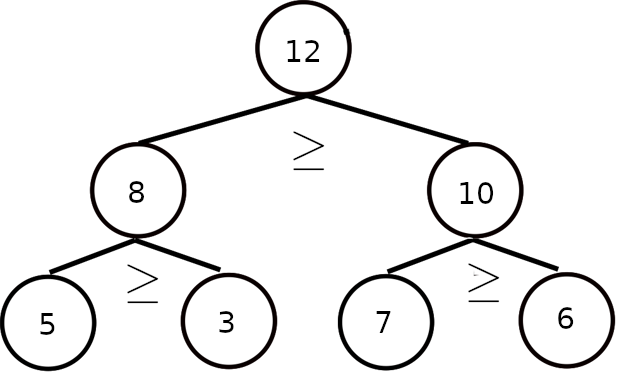
\includegraphics[scale=0.7]{images/heaps_2.png} 
     	%\vspace*{-0.5em}
		%\caption{Floating gate transistor cell}
	\end{figure}
	\end{center}	
	
	
	\column{.5\textwidth}	
	\begin{center}
	\begin{figure}
		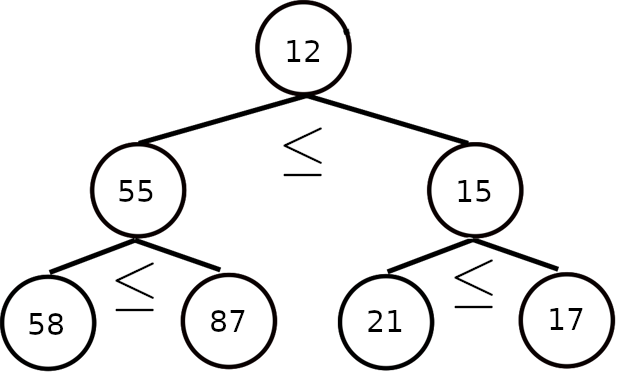
\includegraphics[scale=0.7]{images/heaps_3.png} 
     	%\vspace*{-0.5em}
		%\caption{Floating gate transistor cell}
	\end{figure}
	\end{center}
			
	\end{columns}	
	
	\end{frame}		
	
	\begin{frame}
	
	Interesting properties with binary heaps:
	
	\vspace*{1em}
	
	\begin{itemize}
		\item {Array can be \textit{sorted} using multiple binary heap transformations\footnotemark[4]:
			\begin{enumerate}
				\item {input array is \textbf{transformed into a max binary heap}}
				\item {\textbf{root node value is removed from array} (stored in other final array)}
				\item {a new max binary heap is \textbf{built again from the changed array}}
				\item {\textbf{go to (2)}, until there is no more root nodes}			
			\end{enumerate}				
		}	
		\item {Heap trees can be used as \textit{priority queues}: 
		\begin{itemize}
		\item {Root node contains the \textit{highest priority element}}
		\item {Passing to other lower priority elements: 
		\begin{enumerate}
			\item {\textbf{Removing the root node}}
			\item {\textbf{Rebuilding the heap tree}}
			\item {New highest priority is \textbf{now in the root node, go to (1)}}
		\end{enumerate}
		}
		\end{itemize}}
	\end{itemize}		
	
	\footnotetext[4]{We already saw the heapsort algorithm in course Data Structure 3...}	
	
	\end{frame}		
	
	\section{Binary search trees (BST)}	
	\subsection{Properties}	
	
	\begin{frame}
		
	\begin{block}{What is a \textit{binary search tree}?}
	A \textit{binary search tree} (BST) is:
	\begin{itemize}
		\item {a \textit{\textbf{binary tree}}}
		\item {with the following properties\footnotemark[5] for each node $k$:
			\begin{itemize}
				\item {all nodes $k'$ belonging to \textit{\textbf{left sub-tree}} of $k$:
					\begin{itemize}
						\item {\textbf{values of $k'$ $\leq$ values of $k$}}
					\end{itemize}
				}
				\item {all nodes $k''$ belonging to \textit{\textbf{right sub-tree}} of $k$: 
					\begin{itemize}
						\item {\textbf{values of $k''$ $\geq$ values of $k$}}
					\end{itemize}
				}
			\end{itemize}
		}	
	\end{itemize}		
	\end{block}
	
	\vspace{1em}
	
	Examples of two BSTs:
	
	\vspace*{1em}	
		
	\begin{center}
	
	\begin{figure}
		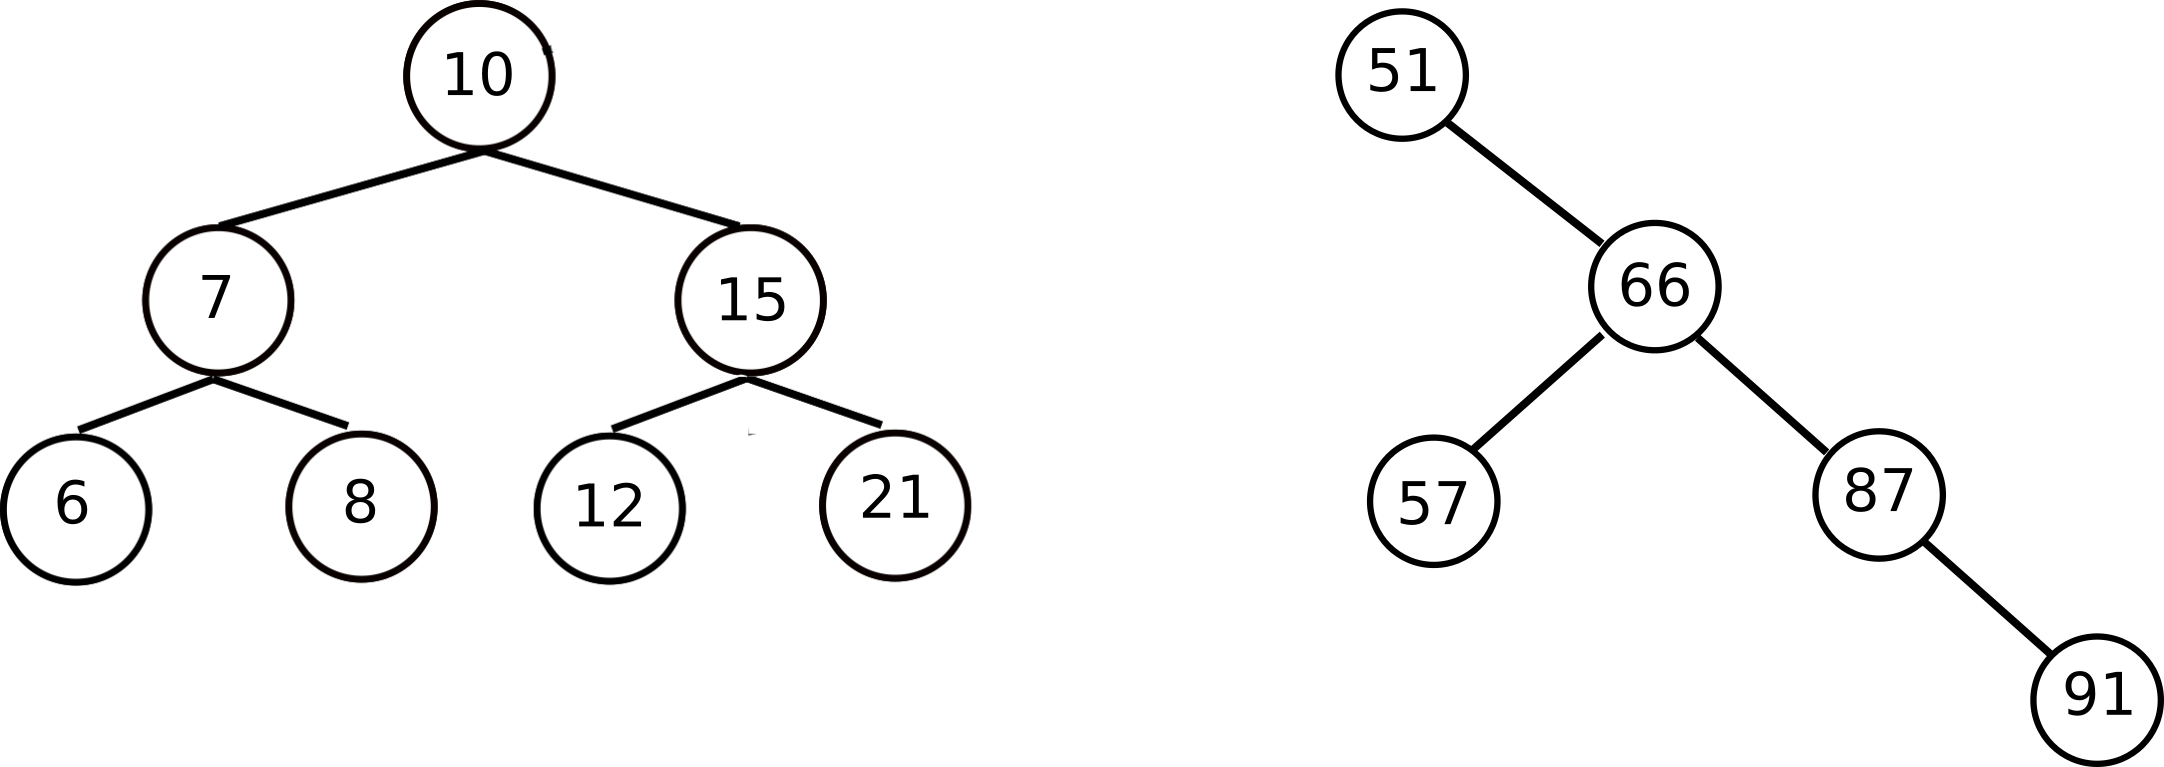
\includegraphics[scale=0.15]{images/binary_search_tree.png} 
     	%\vspace*{-0.5em}
		%\caption{Floating gate transistor cell}
	\end{figure}
	
	\end{center}		
		
	\footnotetext[5]{This also works with values that are not numbers: \textit{there must just be a sorting order}}	
		
	\end{frame}		
	
	\begin{frame}
	
	For searching or inserting in a BST, let's do:
	
	\vspace*{1em}	
	
	\begin{columns}[c]
	\column{.65\textwidth}
	\begin{center}
	\scalebox {0.55} {
	\begin{algorithm}[H]
    \SetAlgoLined   
	\SetKwProg{Fn}{Function}{ is}{end}
	\Fn{$search\_insert(value, address)$} {
		\eIf{$address == NULL$} {
			create\_node(value, address)\;
		} {
			\eIf{$value == address.value$} {
				return address\;
			} {
				\eIf{$value < address.value$} {
					$search\_insert(value, address.left)$
				} {
					$search\_insert(value, address.right)$
				}
			}
		
		}		
	}    

    \end{algorithm}
    }
    \end{center}

	\column{.5\textwidth}	
	Complexities:

	
	\begin{flushleft}
	\scalebox{0.6} {
	\begin{tabular}{c|c|c}
	\textbf{complexities} & \textbf{in average} & \textbf{at worst} \\ \hline
	searching & $O(log(N))$ & $O(N)$ \\ \hline
	inserting & $O(log(N))$ & $O(N)$ \\ \hline
	deleting & $O(log(N))$ & $O(N)$
	\end{tabular}	
	}
	\end{flushleft}	
	
	\end{columns}	
	
	\pause
	
	\begin{block}{Note}
	\begin{itemize}
	\item {\textit{searching}, \textit{inserting} and \textit{deleting} complexities are the same!}
	\item {complexities of \textbf{balanced BSTs are O(log(N))}
		\begin{itemize}
			\item {because searching (as well as inserting and deleting) is dichotomic}
		\end{itemize}			
	}
	\item {complexities of \textbf{badly balanced BSTs are close to O(N)...}}	
	\end{itemize}		
	\end{block}	
	
	\end{frame}		
	
	\begin{frame}
	
	Example of a \textit{badly balanced} BST (left) and a \textit{well balanced} BST (right):
	
	\begin{center}
	\begin{figure}
		
\includegraphics[scale=0.5]{images/balanced_versus_badly_balanced.png} 
     	%\vspace*{-0.5em}
		%\caption{Floating gate transistor cell}
	\end{figure}
	\end{center}	
	
	Both trees have the \textit{same content}, but the \textit{left one is slower to traverse}.
	
	\vspace*{1em}

	\begin{exampleblock}{Definition}
	Each node of a \textit{perfectly balanced} BST verifies:
	\begin{itemize}
		\item {number of nodes in left sub-tree = number of nodes in right sub-tree}
	\end{itemize}		 
	%\begin{itemize}
	%\item {...are \textbf{symmetric} (left and right sub-trees have similar shape)}
	%\item {...have most of their \textit{internal nodes} having \textbf{two child nodes}}
	%\item {...tend to have a \textbf{low high}}
	%\end{itemize}
	\end{exampleblock}	
		
	\end{frame}	
	\section{AVL trees}
	\subsection{Properties}	
	
	\begin{frame}	
	
	\begin{block}{AVL?}
	An \textit{AVL tree} is a \textbf{self-balancing} \textit{binary search tree}
	\end{block}
	
	\vspace*{1em}	
	
	\textit{AVL trees} balance themselves by balancing the \textbf{high of the sub-trees}:
	\begin{itemize}
	\item {do not balance according to the perfectly balanced BST definition}
	\item {\textbf{easier approach} (\textit{much less} computation)}
	\item {good tradeoff}
	\end{itemize}
		
	\vspace*{1em}		
		
	Principle:	
	
	\begin{enumerate}
	\item {once a new node is created: its \textbf{parent nodes are checked}}
	\item {in case there is an unbalanced parent node we \textbf{locally fix it}:
		\begin{itemize}
			\item {addresses of neighbor nodes are \textbf{swapped} so highs are balanced}
			\item {addresses swapping is performed thanks to \textbf{\textit{rotations}}} 
			
		\end{itemize}			
	}
	\end{enumerate}		
	
	\end{frame}	
	
	\subsection{Simple rotation and double rotations}
	
	\begin{frame}
	
	\begin{block}{Rotations?}
	Rotations are elementary AVL operations to \textbf{rebalance the tree}:
	\begin{itemize}
	\item {\textit{unbalanced node}: \textbf{difference between sub-tree highs $\geq$ 2}}
	\item {sub-trees of \textit{unbalanced nodes} are \textbf{rotated}}
	\item {rebalanced nodes \textbf{keep BST properties}}
	\end{itemize}		

	\end{block}
	
	\pause
	
	\vspace*{1em}
	\textit{Simple rotation}\footnotemark[6] (left case):
	
	\begin{center}
	\begin{figure}
		
\includegraphics[scale=0.05]{images/simple_rotation.png} 
     	%\vspace*{-0.5em}
		%\capton{Floating gate transistor cell}
	\end{figure}
	\end{center}	
		
	
	\footnotetext[6]{$A$ is the unbalanced node (high difference $\geq$ 2). $C$ is the newly added node.}	
	
	\end{frame}	
	
	\begin{frame}
	Example of \textit{simple rotation} rebalancing:	
	\vspace*{1em}
	\begin{center}
	\begin{figure}
		
\includegraphics[scale=0.05]{images/simple_rotation_example.png} 
     	%\vspace*{-0.5em}
		%\capton{Floating gate transistor cell}
	\end{figure}
	\end{center}	
		
	\pause		
		
	\begin{block}{Note}
	As you can see: \textit{simple rotation} preserves \textit{BST} properties:
	\begin{itemize}
	\item {the tree is \textbf{still a \textit{binary tree}}}
	\item {all nodes $k'$ belonging to \textit{\textbf{left sub-tree}} of $k$:
				\begin{itemize}
						\item {\textbf{values of $k'$ $\leq$ values of $k$}}
					\end{itemize}
				}
				\item {all nodes $k''$ belonging to \textit{\textbf{right sub-tree}} of $k$: 
					\begin{itemize}
						\item {\textbf{values of $k''$ $\geq$ values of $k$}}
					\end{itemize}
				}	
	\end{itemize}
	\end{block}
	
	\end{frame}	
	
	\begin{frame}
	
	\textit{Double rotation} (left case):
	
	\vspace*{1em}
	
	
	\begin{center}
	\begin{figure}
		\includegraphics[scale=0.045]{images/double-rotation.png} 
     	%\vspace*{-0.5em}
		%\capton{Floating gate transistor cell}
	\end{figure}
	\end{center}	

	

	
	%\begin{block}{Note about this illustration}
	%Here sub-tree highs is max 2 (otherwise the final tree wouldn't be balanced)
	%\end{block}	
	

	\end{frame}
	
	\begin{frame}
	Example of \textit{double rotation} rebalancing:
	\vspace*{1em}	
	
			\begin{center}
	\begin{figure}
		\includegraphics[scale=0.045]{images/double-rotation-example.png} 
     	%\vspace*{-0.5em}
		%\capton{Floating gate transistor cell}
	\end{figure}
	\end{center}	
	
	
	\end{frame}
	
	\begin{frame}
	
		Complexities of a \textit{AVL tree}:

	\vspace*{1em}
	
	\begin{center}
	\scalebox{1} {
	\begin{tabular}{c|c|c}
	\textbf{complexities} & \textbf{in average} & \textbf{at worst} \\ \hline
	searching & $O(log(N))$ & $O(log(N))$ \\ \hline
	inserting & $O(log(N))$ & $O(log(N))$ \\ \hline
	deleting & $O(log(N))$ & $O(log(N))$
	\end{tabular}	
	}
	\end{center}
		
	\end{frame}	

	\section{B-trees}
	
	\subsection{Properties}
	
	\begin{frame}
	
	\begin{block}{B-trees?}
	\textit{B-trees} are also \textbf{self-balancing trees} \textit{but}:
	\begin{itemize}
	\item{unlike \textit{BSTs}, internal nodes \textbf{can have more than 2 child nodes}} 	
	\item{each internal node can have \textbf{k keys and k+1 addresses}}
	\item{\textbf{internal nodes are called pages}}
	\end{itemize}		
	
	\end{block}

	Example of a \textit{B-tree}: 

	
	\begin{center}
	\begin{figure}
		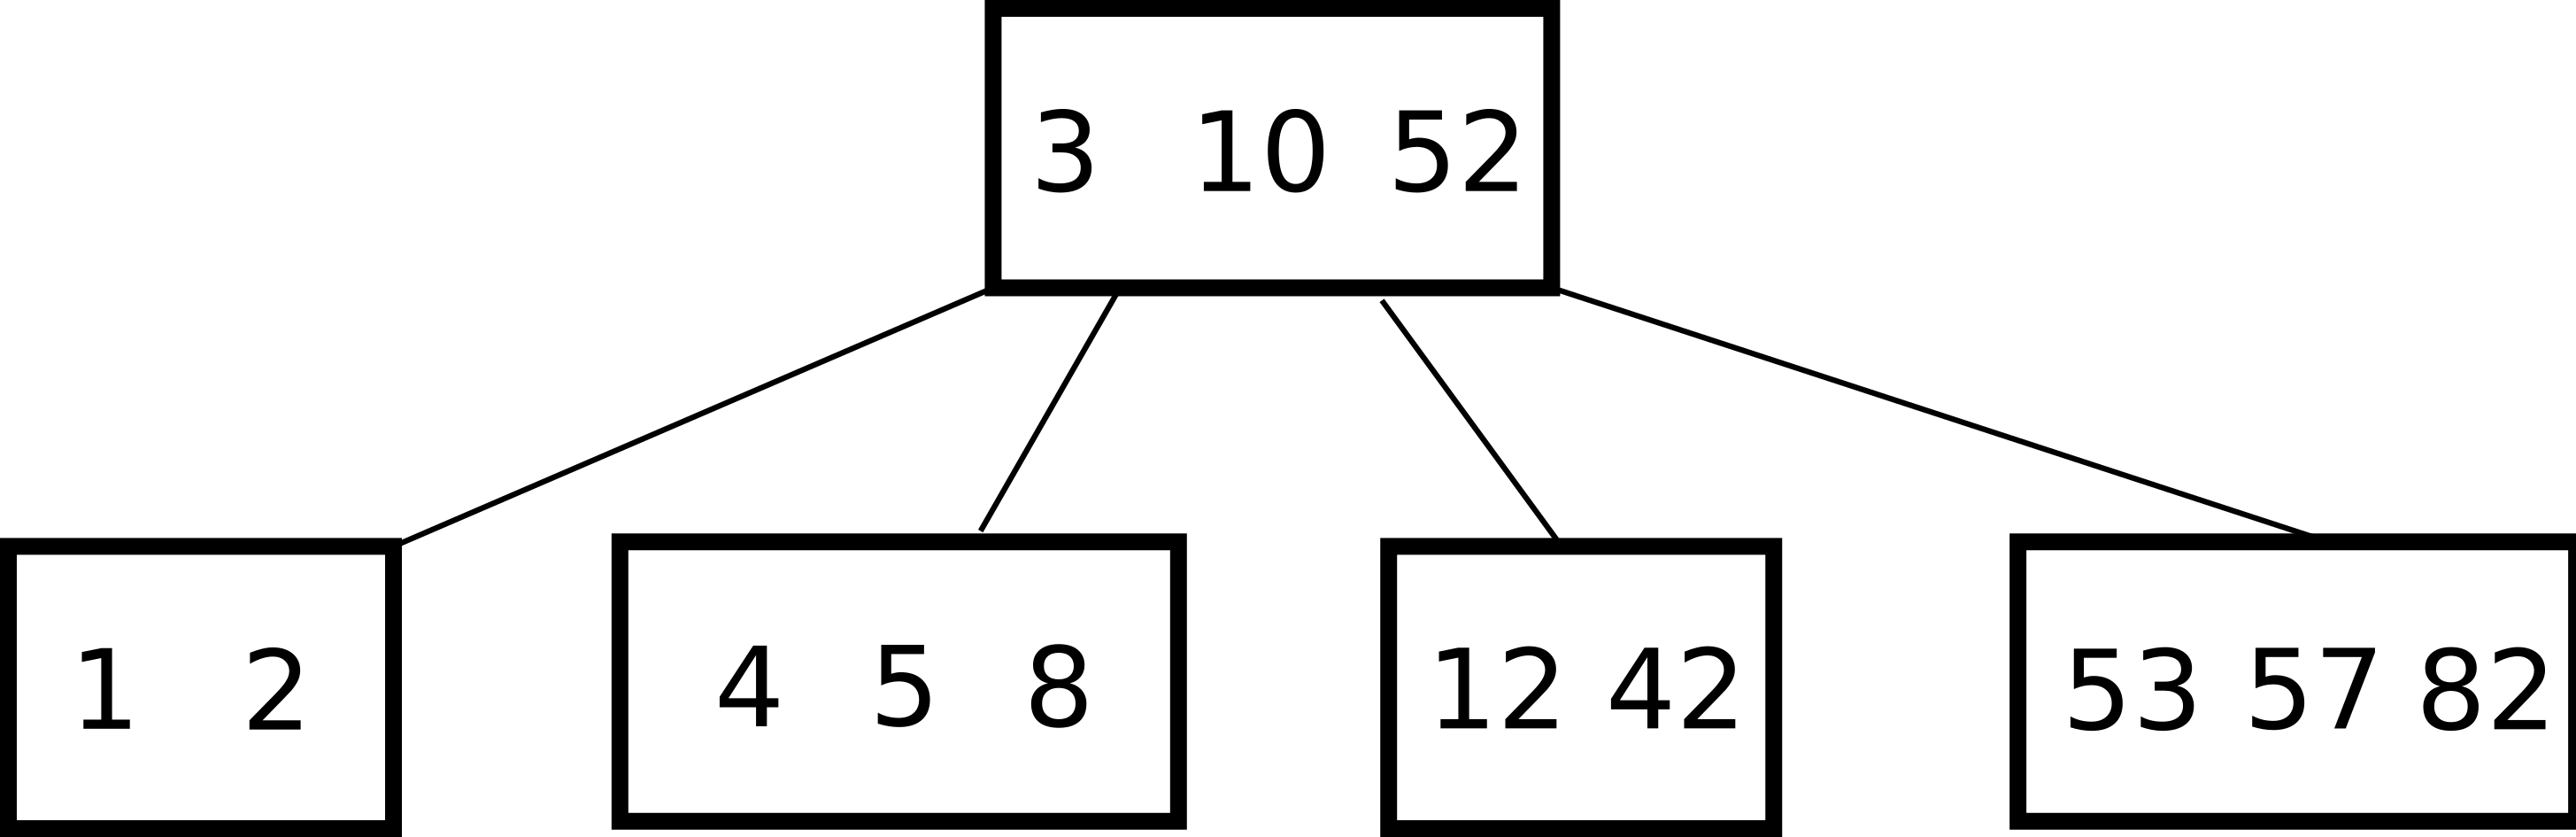
\includegraphics[scale=0.1]{images/b-trees.png} 
     	%\vspace*{-0.5em}
		%\capton{Floating gate transistor cell}
	\end{figure}
	\end{center}	

	\pause

	\begin{block}{Note}
	\textit{B-trees} are interesting for \textbf{for reading and writing large blocks of data}\footnotemark[11]
	\end{block}


	\footnotetext[11]{Example of applications using it: \textit{databases} and \textit{file systems}. Here, most of the time, the number of keys cannot fit main memory: but \textit{B-trees} allow to search efficiently in large blocks of data with few memory accesses (= few keys in main memory). Very often: B-tree node size = disk block size.}

	
	\end{frame}	

	\begin{frame}
	
	\textit{B-trees} are built as follows:
	
	\begin{center}
	\begin{figure}
		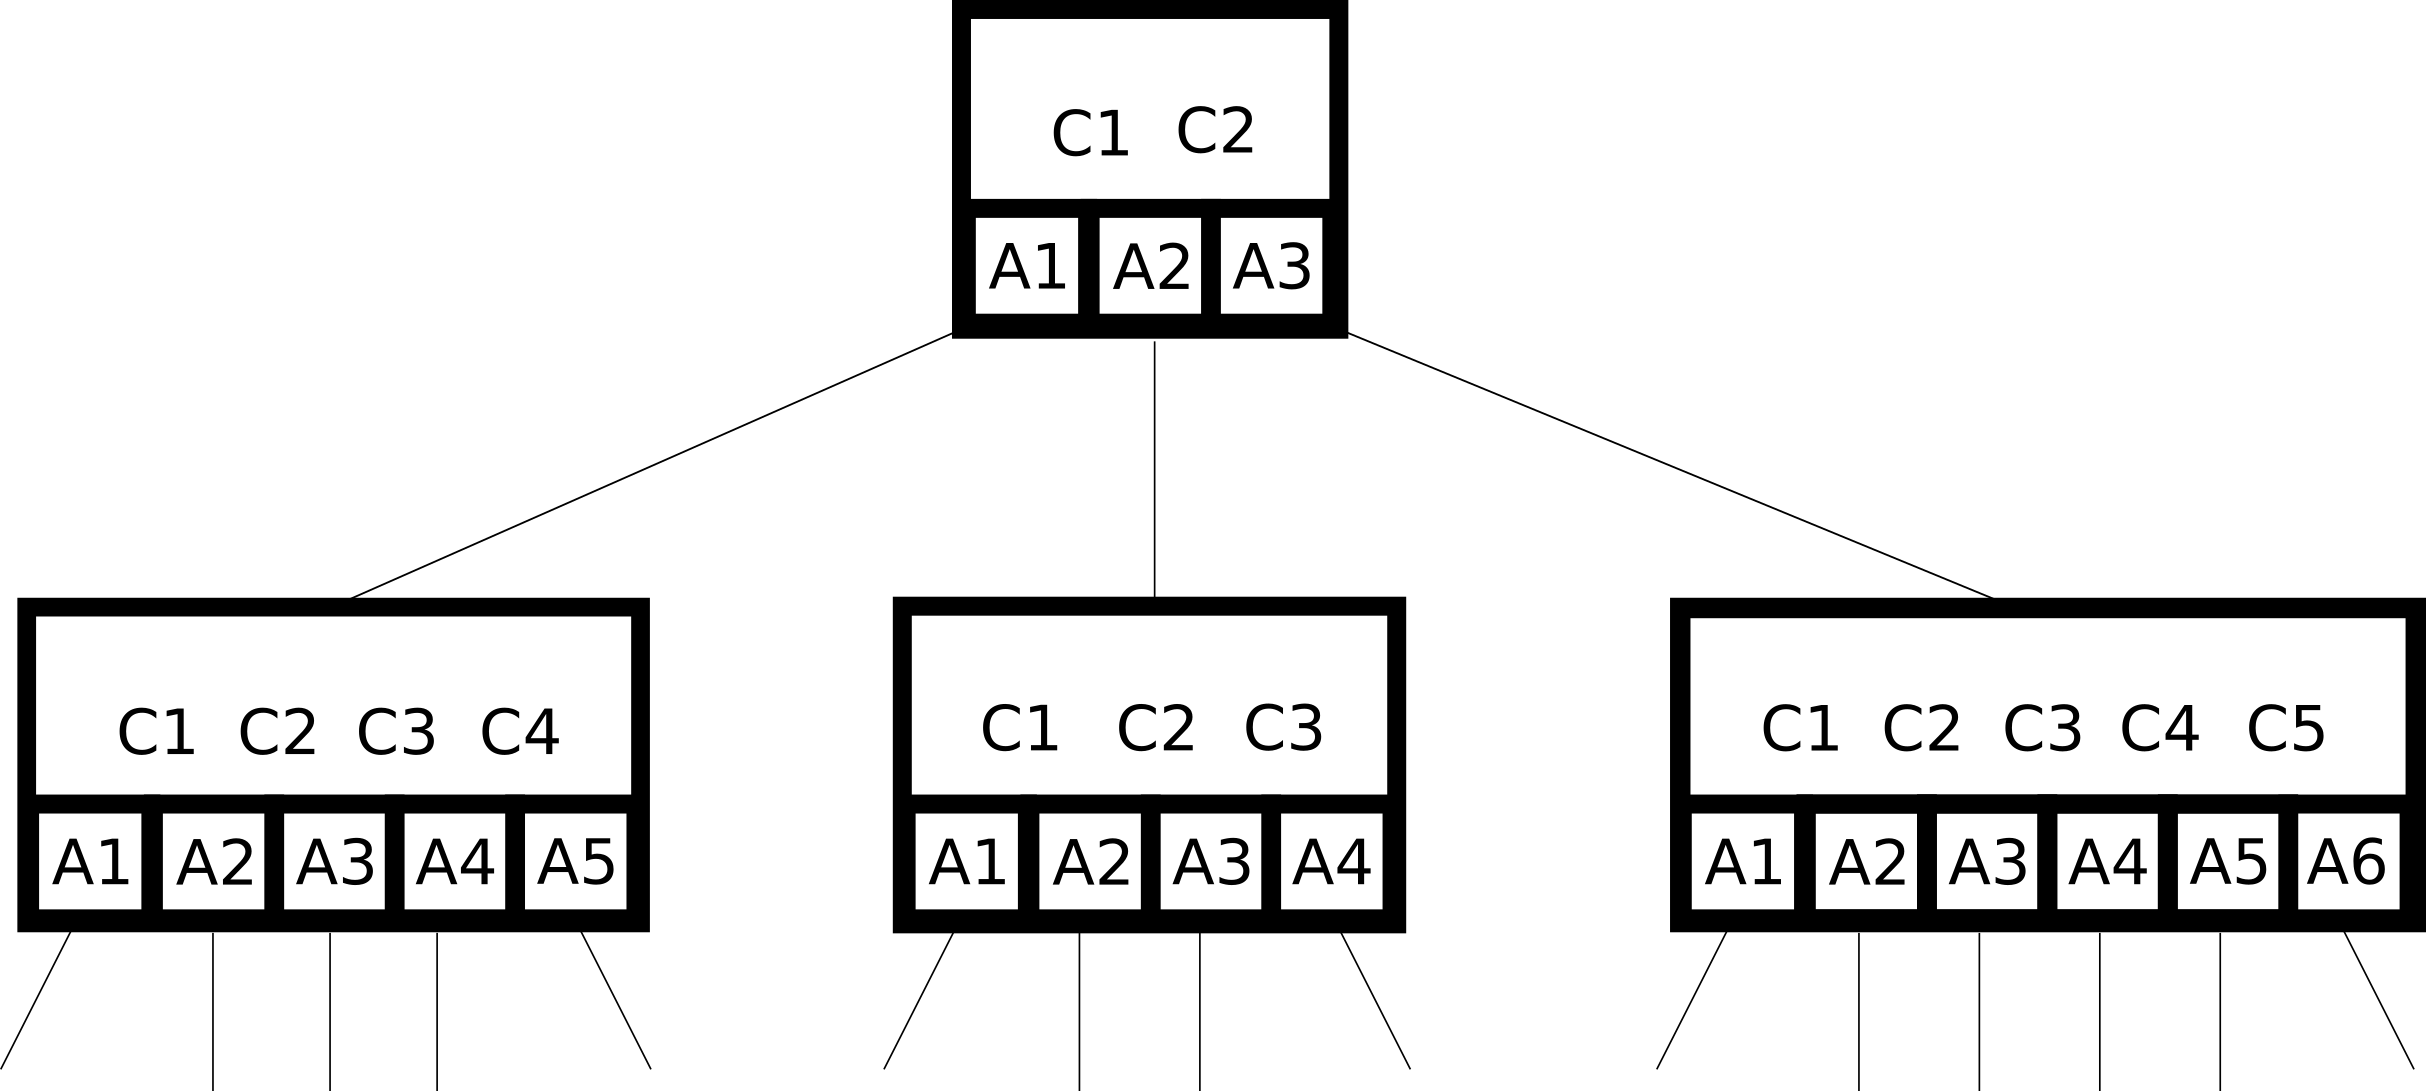
\includegraphics[scale=0.2]{images/b-trees-explicit.png} 
     	%\vspace*{-0.5em}
		%\capton{Floating gate transistor cell}
	\end{figure}
	\end{center}
	
	
	\begin{itemize}
	\item {For each node, \textbf{keys are ordered}: C1 < C2 < C3 < C4...}
	\item {Splits are organized like a generalized \textit{BST}, example for the first page:
		\begin{itemize}
			\item {keys < key C1 belong to the node pointed by A1}
			\item {keys > key C3 and < C4 belong to the node pointed by A4}
		\item {keys > key C4 belong to the node pointed by A5  }
		\end{itemize}
	}
	\end{itemize}		
	
	\pause	
	
	\begin{exampleblock}{B-tree of order N}
	N minimum number of keys and $2\times N$ maximum number of keys per page
	\end{exampleblock}	
		
	\end{frame}

	\begin{frame}

	Searching a key in a \textit{B-tree} is quite easy, for example:
	
	\vspace*{1em}
	
	\begin{itemize}
	\item {Where is 5? I know that 3 < 5 < 10: I follow address A2}
	\item {Where is 42? I know that 10 < 42 < 52: I follow address A3}
	\item {Where is 57? I know that 57 > 52: I follow address A4}
	\item {...}
	\end{itemize}
		
	\begin{center}
	\begin{figure}
		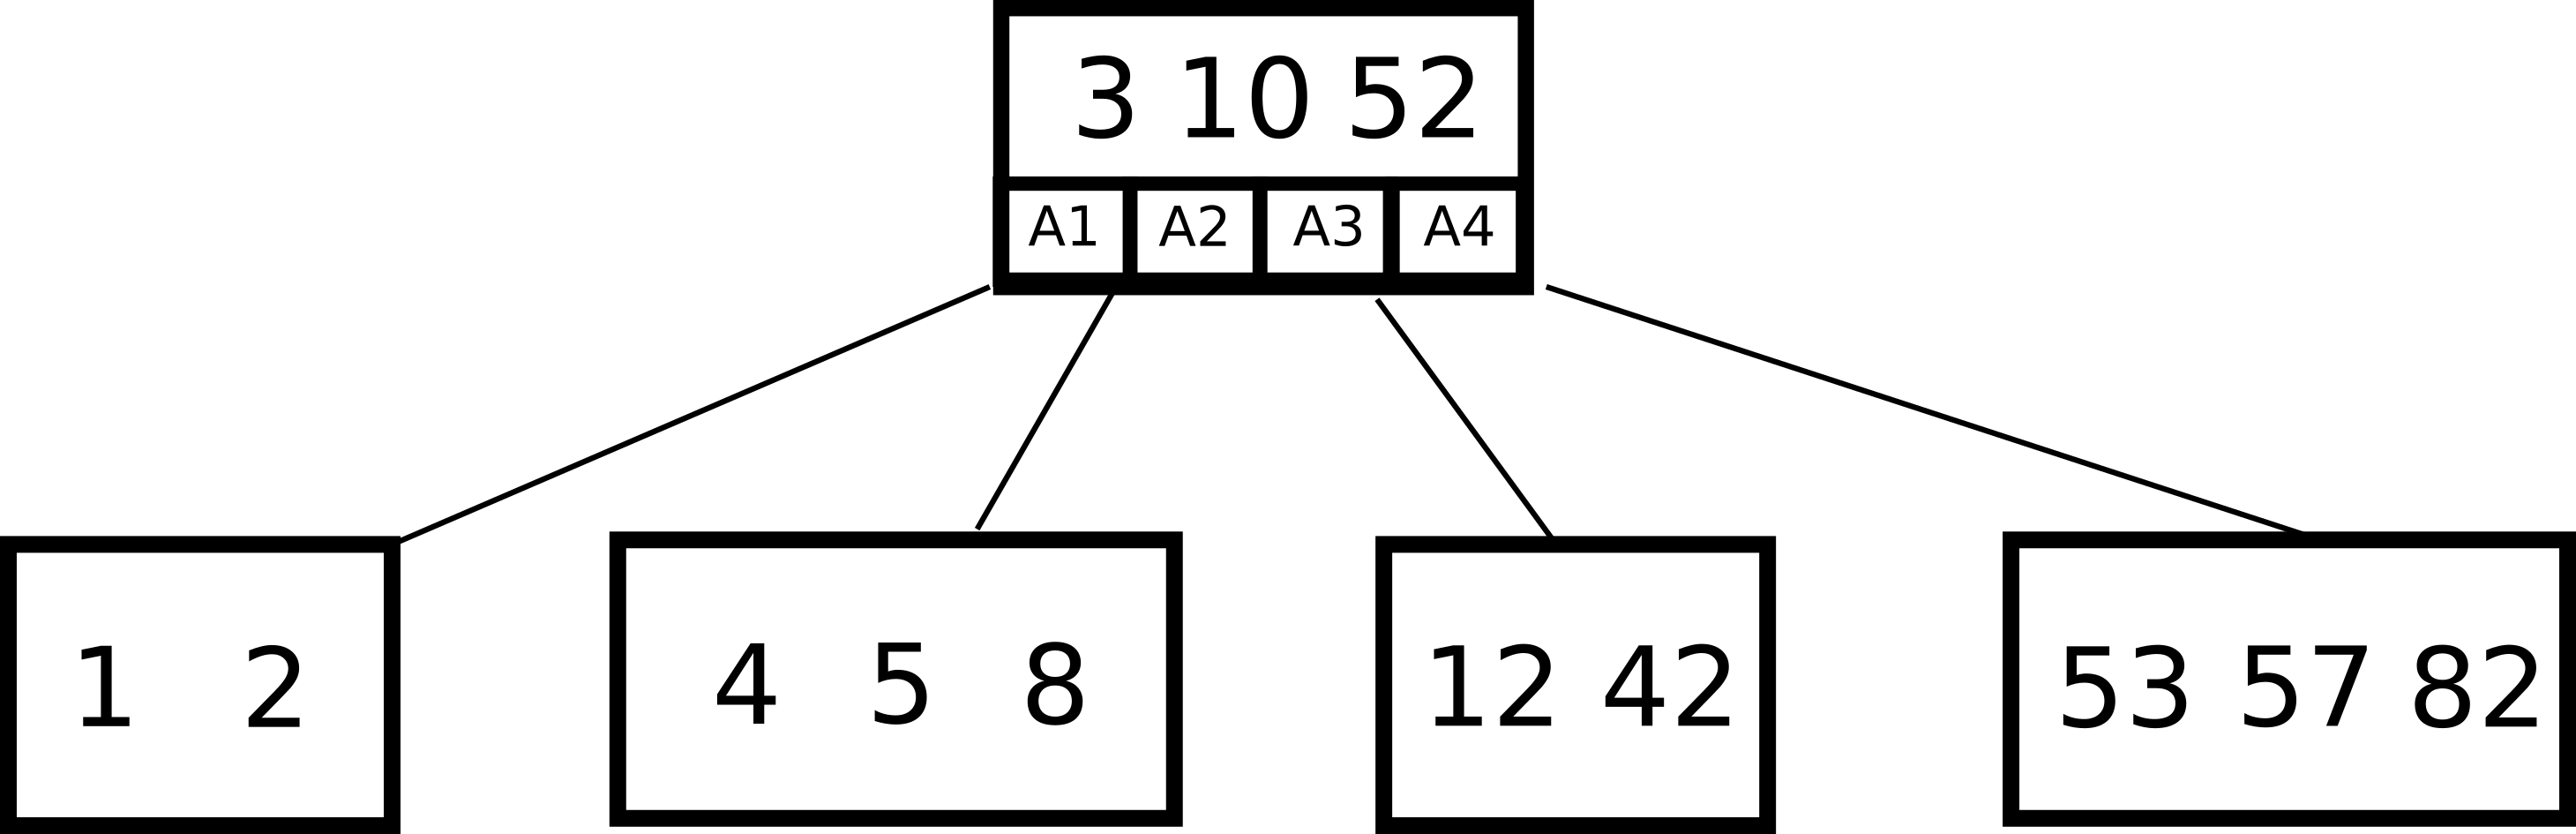
\includegraphics[scale=0.2]{images/b-trees-2.png} 
     	%\vspace*{-0.5em}
		%\capton{Floating gate transistor cell}
	\end{figure}
	\end{center}	
	
	\end{frame}	
		
	\begin{frame}
	
	Examples of key insertions in a \textit{B-tree} of order 2:
	
	\vspace*{1em}	
	
	In a \textit{non saturated leaf node}:	
	
	\vspace*{1em}
	
		\begin{center}
	\begin{figure}
		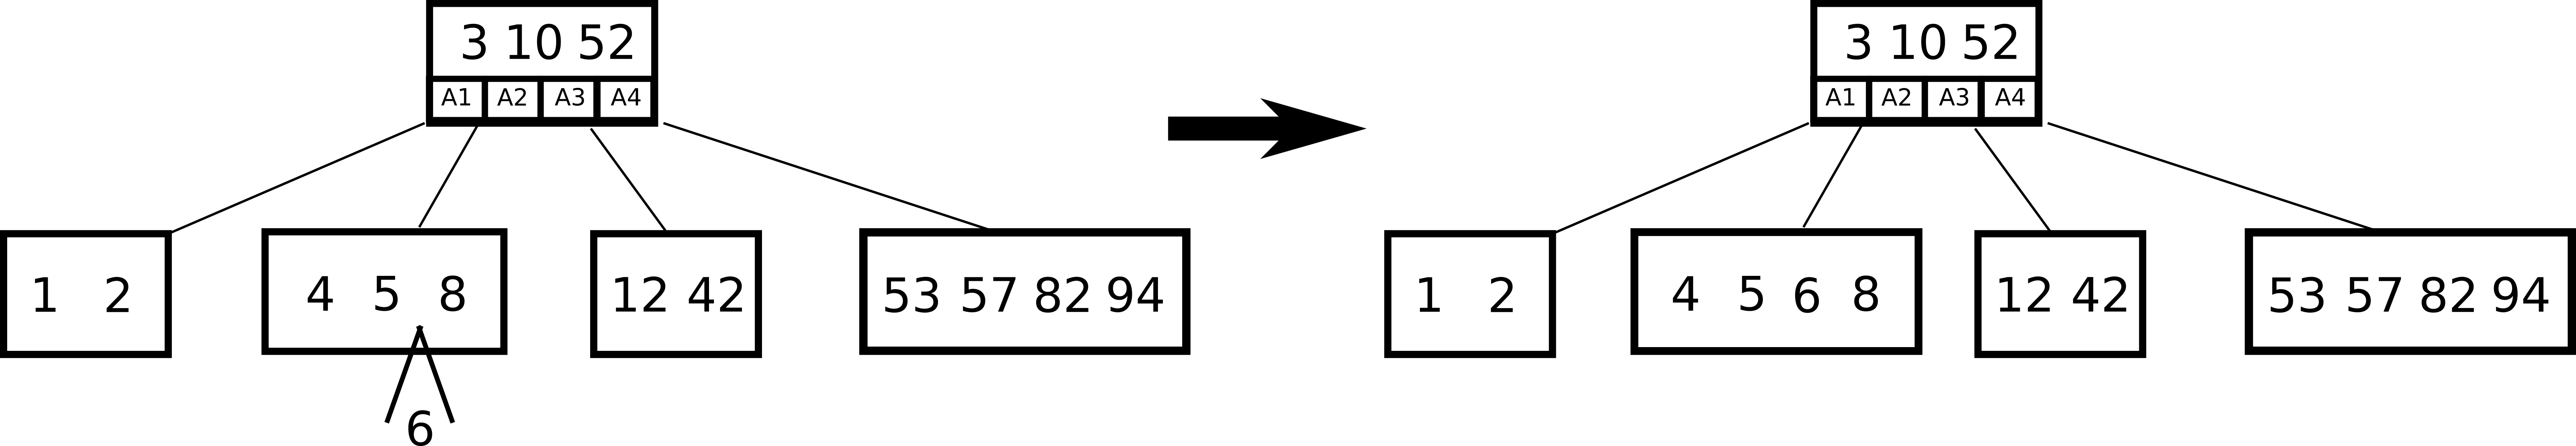
\includegraphics[scale=0.1]{images/b-trees-insert-1.png} 
     	%\vspace*{-0.5em}
		%\capton{Floating gate transistor cell}
	\end{figure}
	\end{center}	
	
	In a \textit{saturated leaf node} (B-tree order 2: max number of keys = 4):
		
	\begin{center}
	\begin{figure}
		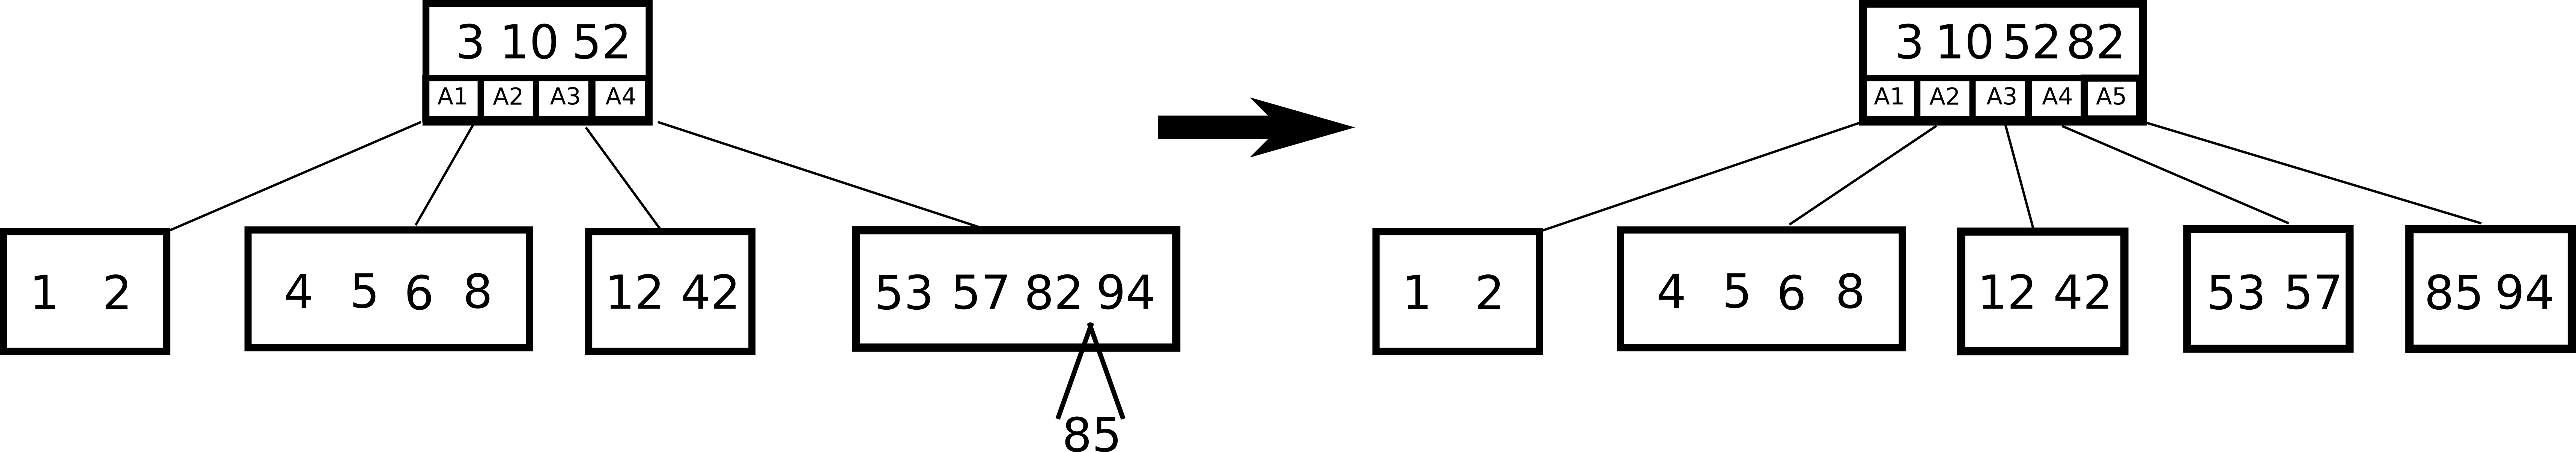
\includegraphics[scale=0.1]{images/b-trees-insert-2.png} 
     	%\vspace*{-0.5em}
		%\capton{Floating gate transistor cell}
	\end{figure}
	\end{center}	
	
	
	\end{frame}	
	
	\begin{frame}
	
	In a saturated node with a saturated root node:	
	
	\vspace*{1em}	
	
	\begin{center}
	\begin{figure}
		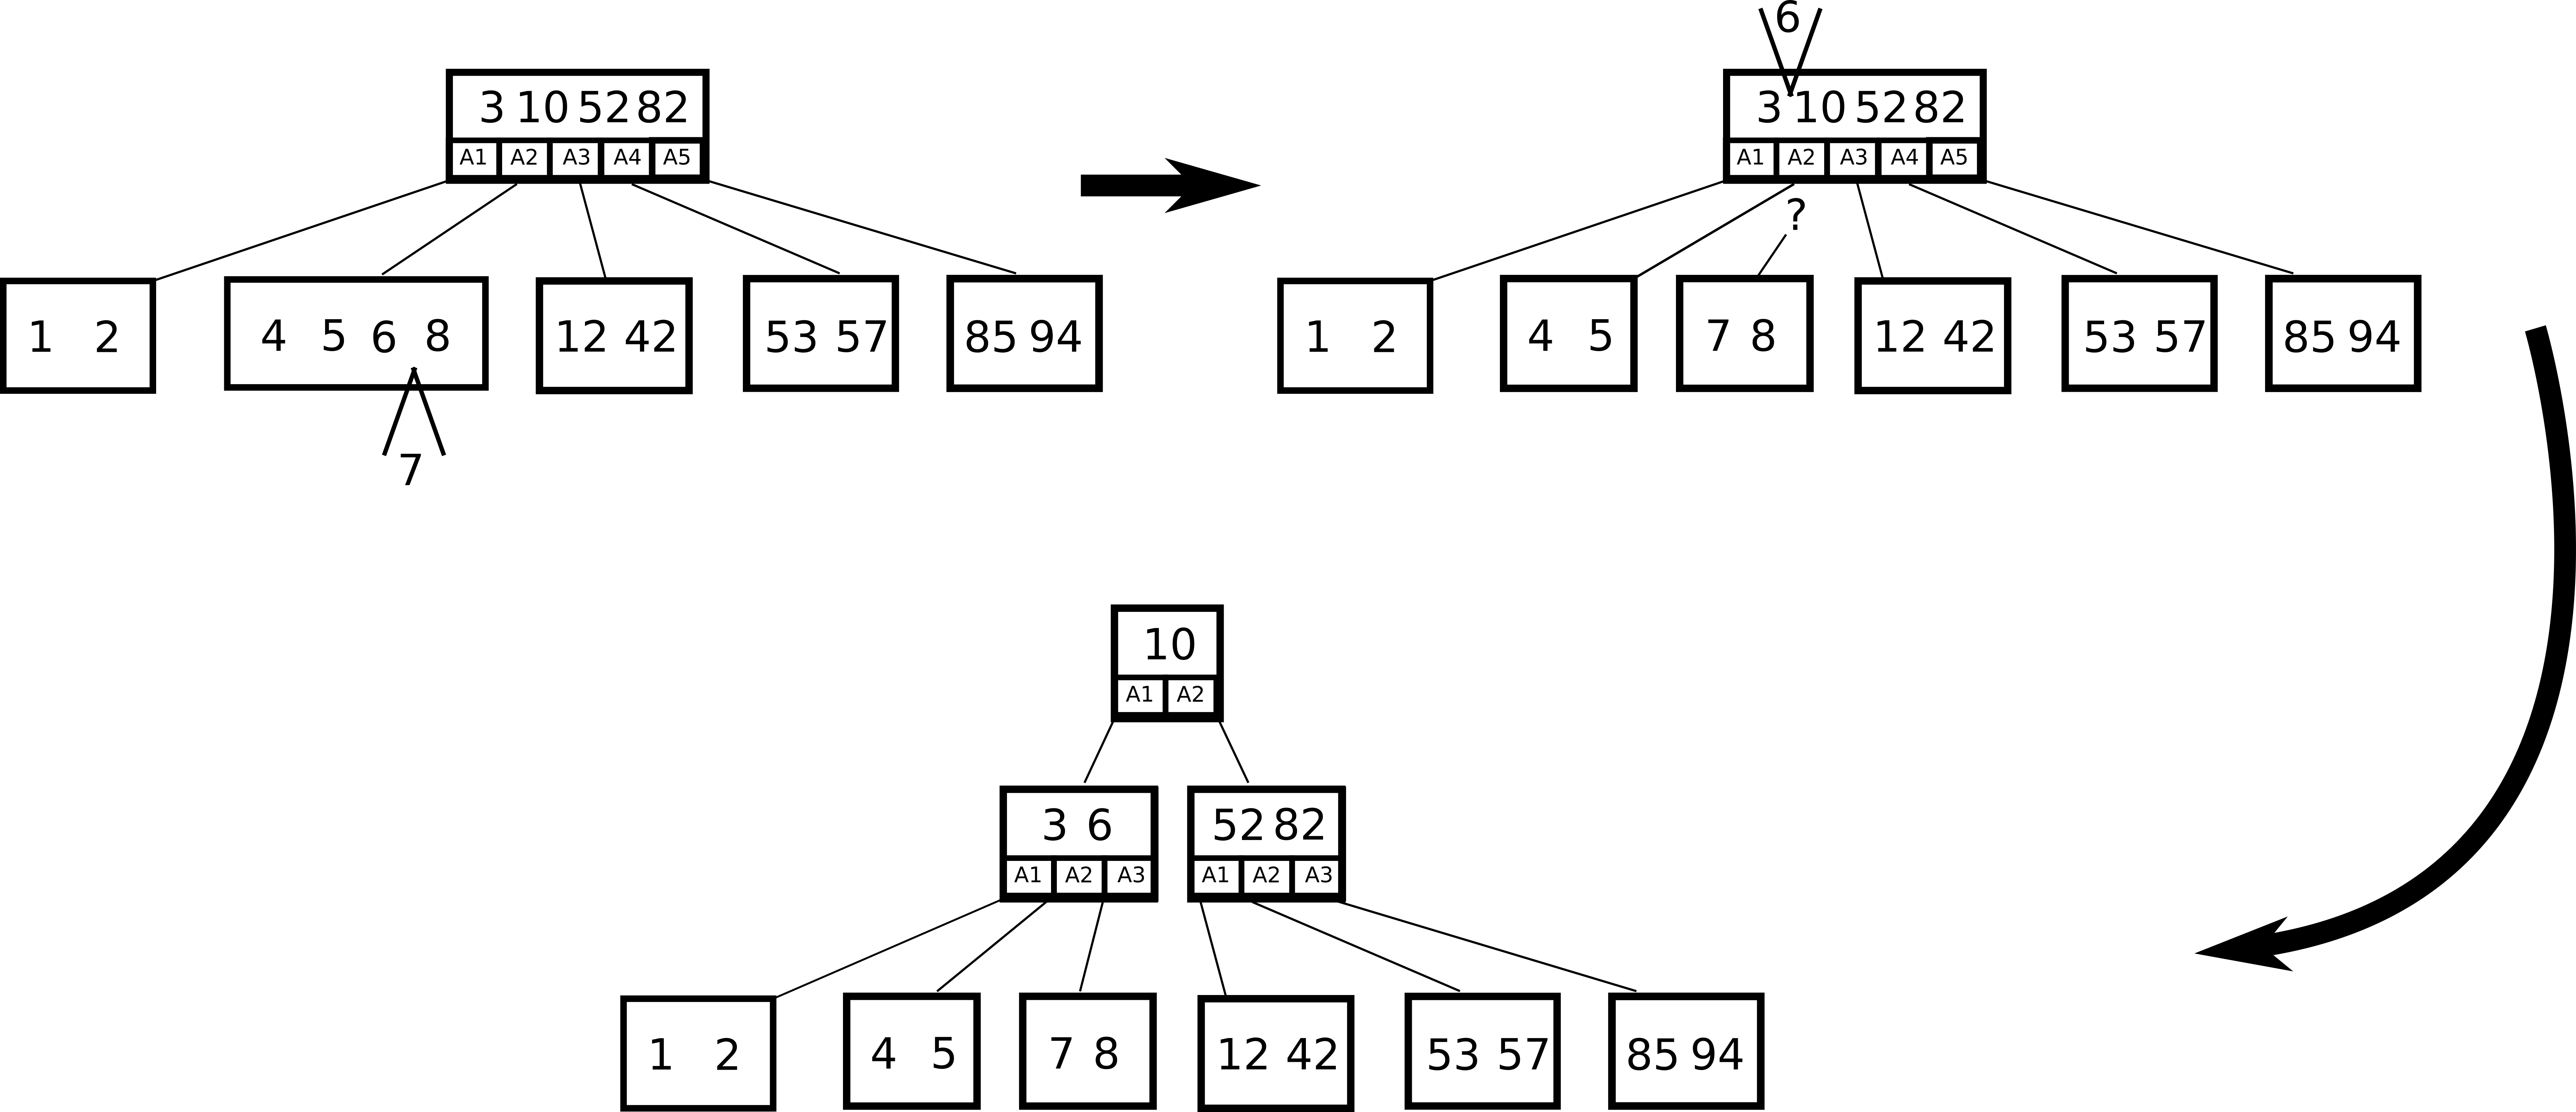
\includegraphics[scale=0.1]{images/b-trees-insert-3.png} 
     	%\vspace*{-0.5em}
		%\capton{Floating gate transistor cell}
	\end{figure}
	\end{center}		
	
	
	\end{frame}	
	
	\begin{frame}
	
	Complexities of a \textit{B-tree}:

	\vspace*{1em}
	
	\begin{center}
	\scalebox{1} {
	\begin{tabular}{c|c|c}
	\textbf{complexities} & \textbf{in average} & \textbf{at worst} \\ \hline
	searching & $O(log(N))$ & $O(log(N))$ \\ \hline
	inserting & $O(log(N))$ & $O(log(N))$ \\ \hline
	deleting & $O(log(N))$ & $O(log(N))$
	\end{tabular}	
	}
	\end{center}
		
	\end{frame}		
	
	
	\section{Summary}
	
	\begin{frame}
	
	\begin{itemize}
	\item {\textit{Complete and half complete binary trees} $\Leftrightarrow$ arrays}
	\item {\textit{Binary heaps}: useful structure for \textbf{sorting} and \textbf{priority queues}}
	\item {\textit{Binary search trees}:
		\begin{itemize}
			\item {if \textbf{well-balanced}: \textbf{best insertion/deletion/reading complexities}}
			\item {\textbf{badly balanced}: complexities \textbf{close to those of linked-list}}
		\end{itemize}	
	}	
	\item {\textit{AVL trees}:
		\begin{itemize}
			\item {\textit{BST} with \textbf{self-balancing properties}}
			\item {\textbf{best insertion/deletion/reading complexities}}
		\end{itemize}			
	}	
	\item {\textit{B-trees}:
		\begin{itemize}
			\item {well suited for large blocks of data (nodes can have > 2 children)}
			\item {sort of \textbf{generalized \textit{BST}} (it's not binary! despite the "B-" prefix)}
			\item {\textbf{self-balancing}}
			\item {\textbf{best insertion/deletion/reading complexities}}
		\end{itemize}
	}
	\end{itemize}
	
	
	
	

	
	\end{frame}
	



\end{document}